\section{Results and Discussion} \label{sec:results}

\subsection{Gene Duplication Facilitates Adaptive Evolution}

In a first set of experiments, we set out to whether slip duplications affect adaptive evolution of Logic-9 phenotypes in our study system.
Comparing slip-duplicate-enabled and baseline treatments, we found slip duplications to yield significantly higher evolved phenotypic adaptation scores (two-tailed Mann-Whitney U test, $W = 562.5$, Bonferroni-adjusted $p << 0.0001$; Figure \ref{fig:results_panels}; first-phase experiments).

This result aligns with existing findings across a broad variety of biological taxa and digital models that slip-duplication of genetic material can facilitate evolution of adaptive traits \citep{Koza:1995fr,Zhang:2003fw,Teichmann:2004cz}.
Indeed, in earlier-reported experiments, we found gene duplication mechanisms to also facilitate adaptive evolution in changing environments, where the set of rewarded tasks fluctuated across generations \citep{lalejini2017gene}.

\begin{figure}[!h]
  %\centering
  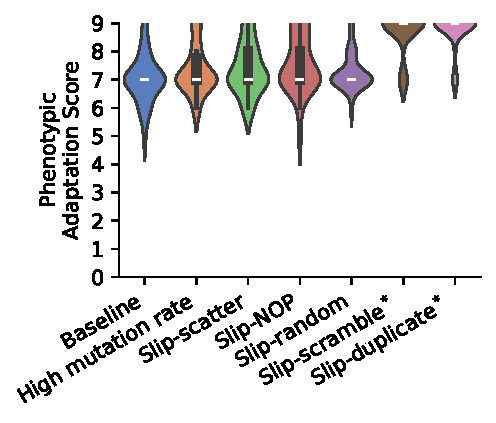
\includegraphics[height=2in,trim={0.2cm 0 0.2cm 0},clip]{binder/binder/teeplots/env=static+hue=treatment+inner=box+kind=violin+palette=muted+viz=catplot+x=treatment+y=tasks-present+ext=.pdf}%
   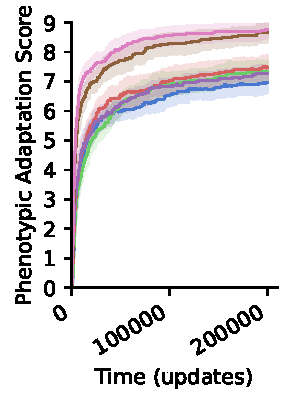
\includegraphics[height=2in,trim={0.94cm -0.64cm 0 0},clip]{binder/binder/teeplots/env=static+errorbar=ci+hue=treatment+kind=line+palette=muted+viz=relplot+x=time+y=tasks-present+ext=.pdf}

   \vspace{-2ex}

  \caption{\textbf{Slip-scramble and slip-duplicate treatments facilitate adaptive evolution.}
  \small Violin plots indicate the phenotypic match scores for final dominants.
  Each time series shows the phenotypic match scores for the lineages of final dominant organisms over time. The colors in each time series correspond to the colors in the violin plots.
  Treatments that have significantly higher phenotypic match scores than the baseline treatment are marked with *.
  Data shown from second-phase experiments.
}
  \label{fig:results_panels}
\end{figure}


\subsection{Sequence Content of Duplications Contribute to Adaptive Evolution}

Having observed that slip-duplicate mutations accelerate evolution of Logic-9 phenotypes, we next sought to isolate the aspects of slip duplication contributing to adaptation.
For this purpose, we tested four variants of the slip-duplication operator disabling or replacing a particular aspect of slip duplication (overviewed in Figure \ref{fig:slip_mut_variants}.)

As shown in Figure \ref{fig:results_panels}, we detected benefits to adaptive evolution only for the follow-up slip-scramble treatment --- which randomized sequence order within duplicated regions (two-tailed Mann-Whitney U test; Figure \ref{fig:results_panels}; first-phase experiments).
Phenotypic adaptation scores under all other slip-duplicate variants were indistinguishable or slower-adapting compared with the baseline treatment.

Given the efficacy of the slip-scramble treatment in facilitating adaptation, we additionally tested whether phenotypic adaptation differed between the slip-scramble and full-fledged slip-duplicate operators.
To prevent issues with multiple comparisons, we dispatched 100 new trials under both treatments for this test.

% p = 0.011
We found that the slip-duplicate treatment did, in fact, yield higher task counts compared to the slip-scramble treatment (two-tailed Mann-Whitney U test, $W = 4305$ respectively, Bonferroni-adjusted $p < 0.02$; first-phase experiments).
These results indicate that both content and structure of duplicated genetic material contribute to facilitating adaptive evolution.

As above, earlier-reported experiments within our study system concur with present work, finding sequence content and order to both also benefit adaptive evolution within changing environments \citep{lalejini2017gene}.

\subsection{How Does Slip Duplication Facilitate Adaptive Evolution?}

Thus far, we have established slip-duplications of genetic material can significantly benefiut adaptive evolution, and that sequence content and order both contribute to this effect.
We next sought to explain \textit{how} the structural characteristics of slip duplications promote adaptive evolution in our study system.

In these investigations, we evaluated three hypotheses around evolutionary dynamics of slip duplications.
First, we explored how the facilitation of adaptive evolution by gene duplication differed between simple and complex traits promoted by gene duplication.
Second, we tested for signatures of evolutionary potentiation by gene duplications along lineage histories.
Finally, we examined how slip duplication influences genetic architecture with respect to brittleness and vestigial genetic material.

\subsubsection{Slip Duplication Facilitates the Evolution of Complex Traits}

\begin{figure*}
    \centering
    \begin{subfigure}{\textwidth}
    \includegraphics[width=\linewidth,trim={0 13cm 0 0},clip]{binder/binder/teeplots/adaptive-evolution-rate.ipynb/col=components+errorbar=ci+hue=treatment+kind=line+post=plt-xlim-0-600+row=mutation+viz=relplot+x=generation+y=has-task+ext=.pdf}
\includegraphics[width=\linewidth,trim={0 0 0 24cm},clip]{binder/binder/teeplots/adaptive-evolution-rate.ipynb/col=components+errorbar=ci+hue=treatment+kind=line+post=plt-xlim-0-600+row=mutation+viz=relplot+x=generation+y=has-task+ext=.pdf}
    \caption{\footnotesize including directly-facilitated adaptive variation from slip duplication (tasks gained directly through slip duplication); (blue: long-ancestor; purple: baseline treatment; orange: slip-duplicate treatment)}
    \label{fig:adaptive-evolution-rate:direct}
    \end{subfigure}

    \begin{subfigure}{\textwidth}
\includegraphics[width=\linewidth,trim={0 0 0 13cm},clip]{binder/binder/teeplots/adaptive-evolution-rate-nodirect.ipynb/col=components+errorbar=ci+hue=treatment+kind=line+post=plt-xlim-0-600+row=mutation+viz=relplot+x=generation+y=has-task+ext=.pdf}
    \caption{\footnotesize excluding directly-facilitated adpative variation from slip duplication (only instances where tasks did not arise as an immediate consequence of slip duplication); (brown: long-ancestor; purple: baseline treatment; red: slip-duplicate treatment)}
    \label{fig:adaptive-evolution-rate:nodirect}
    \end{subfigure}
    \caption{
        \textbf{Rate of adaptive evolution across a spectrum of task complexities.}
        \footnotesize
        Simple tasks (leftmost panels) require only one logic gate component.
        More complex tasks (rightmost panels) require up to five logic gate components.
        Slip-duplication treatment facilitates significantly faster adaptive evolution than long-genome treatment for more complex tasks, requiring 4 or 5 components (top panel).
        Without instances where tasks were acquired directly through slip duplicaiton, however, no significant difference is detected between the adaptive rates of long-genome and slip-duplication treatments for these more complex tasks (bottom panel).
        Error bands give 95\% CI, bootstrapped over 30 replicates per treatment.
    }
    \label{fig:adaptive-evolution-rate}
\end{figure*}


One limitation of our first-phase experiments was in not directly testing the influence of genome length on adaptive evolution.
Although tested slip-duplication variants provided opportunity for growth in gemone length, large genome size was not itself directly enforced.
For this reason, we incorporated an additional ``long-genome'' control treatment initialized with a 1,000-site ancestor (rather than 100-site) into our second-phase experiments.

Comparing the long-genome and baseline treatments, we observed genome length alone to significantly boost task acquisition.
Disaggregating by task complexity, though, reveals  impact of genome length as most prominent in the acquisition of simple tasks.
Figure \ref{fig:adaptive-evolution-rate} compares acquisition rates for tasks across task complexity classes --- with and without slip duplication, including the long-genome control.
The long-genome control matched or exceeded the performance of slip-duplication in evolving simple traits with 3 or fewer components.
% https://github.com/chaynes2019/AvidaGeneDupe/blob/538ede79c7301f10718ca96c8dd38782b6882632/binder/adaptive-evolution-rate.ipynb
However, slip duplication evolved more complex 4- and 5-component traits within a significantly higher fraction of replicates compared to the long-genome control (Fisher's exact tests; 36/60 vs. 24/60, $p<0.05$ [4 components]; 10/30 vs. 2/30, $p<0.03$ [5 components]; second-phase experiments; Figure \ref{fig:adaptive-evolution-rate}).
This behavior is noteworthy in lending empirical evidence to longstanding theory hypotehsizing gene duplication as a catalyst for evolution of complex traits \citep{ohno1970evolution}.

\subsubsection{Slip-Duplicated Regions Potentiate Coding Sites for Novel Complex Traits}

% https://github.com/chaynes2019/AvidaGeneDupe/blob/4c7fa27229094adcb5bdb0b1aec541d0014b0fed/binder/hard-task-gain.ipynb
%             H-statistic       p-value
% Components
% 1              1.011820  3.144672e-01
% 2             22.787798  1.809107e-06
% 3             33.846753  5.962854e-09
% 4             15.359894  8.885441e-05
% 5              9.097744  2.559249e-03
%    Components  Prev Slip Insertion Cumulative Count      mean       std
% 0           1                                 False  0.932088  0.455109
% 1           1                                  True  1.002025  1.164197
% 2           2                                 False  0.588566  0.618479
% 3           2                                  True  1.579974  1.191681
% 4           3                                 False  0.491481  0.700256
% 5           3                                  True  1.516115  0.911430
% 6           4                                 False  0.703793  0.980105
% 7           4                                  True  1.229158  0.654042
% 8           5                                 False  0.583674  0.927917
% 9           5                                  True  1.249985  0.531423
%    Components  Prev Slip Insertion Cumulative Count  size
% 0           1                                 False    60
% 1           1                                  True    48
% 2           2                                 False    60
% 3           2                                  True    56
% 4           3                                 False    60
% 5           3                                  True    59
% 6           4                                 False    52
% 7           4                                  True    52
% 8           5                                 False    20
% 9           5                                  True    20

\begin{figure}
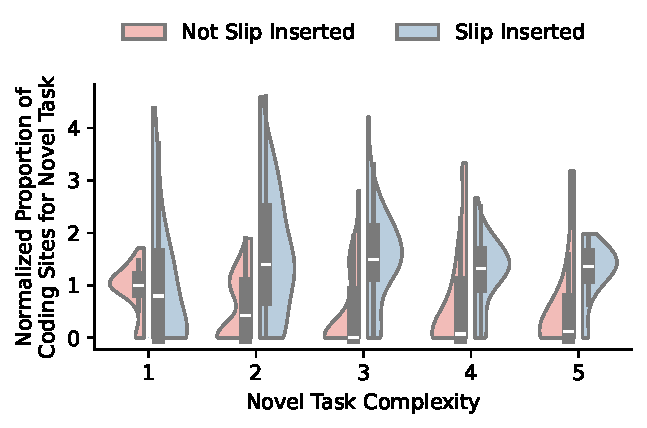
\includegraphics[
width=\linewidth
]{binder/binder/teeplots/density-norm=width+hue=prev-slip-insertion-cumulative-count+kind=violin+viz=catplot+x=components+y=is-task-coding-site+ext=.pdf}
\caption{%
  \textbf{Slip-duplicated sites are overrepresented among \textit{de novo} coding sites for complex traits.}
  \footnotesize
  Distributions compare frequencies of previously slip-duplicated and non-slip-duplicated sites among  \textit{de novo} task coding sites, normalized to neutral expectation.
  Values greater than 1 indicate that sites are overrepresented among the coding sites of novel traits compared to their background frequency.
  Differences between slip-duplicated and non slip-duplicated sites are significant for tasks requiring 2 or more NAND components (Mann-Whitney test; $p < 0.01$).
} \label{fig:potentiation}
\end{figure}


Thus far, we have established that slip duplication promotes evolution of novel traits within our study system, and that this facultative effect biases towards complex traits.
We next sought to characterize aspects of genetic architecture through which slip duplication drives adaptation.
In particular, we sought to understand whether genetic material introduced through slip duplication itself is potentiated to code for novel adaptive traits.
For each first occurrence of a phenotype arising in sample final-dominant lineages, we assessed the density of coding sites for new tasks in genome regions that had previously been slip duplicated.
Figure \ref{fig:potentiation} compares involvement in coding for new tasks between previously slip-duplicated and non-slip-duplicated sites.
For the simplest tasks, requiring only one NAND component, we found no significant difference in the likelihood of duplicated sites participating in coding regions for new tasks.
% https://github.com/chaynes2019/AvidaGeneDupe/blob/2d31c0bd0cc9bdbf4bb49224859d6bd165cd36c8/binder/hard-task-gain2.ipynb
However, we found significant associations for traits with two or more NAND components (one-sample Wilcoxon signed-rank tests; $n=56,59,52,20$ observations; second-phase experiments).
Effect sizes of potentiation on likelihood to code for novel traits were $1.6\times$, $1.6\times$, $1.2\times$, and $1.2\times$ respectively for 2, 3, 4, and 5 task components.
Smaller effect sizes at 4- and 5-component tasks may be due to a larger portion of the genome becoming comprised of slip-duplicated sites (Supplementary Figure \ref{fig:potentiation-supp}), thus lowering the upper ceiling on deviation from expected.

One possible confounding factor in this result is evolutionary constraint at genome sites involved in organsims' self-replication loop.
These sites are critical to viability, with lethal outcomes when knocked out.
We found that these critical sites were less likely to be involved in slip duplication and also less likely to be involved in coding for \textit{de novo} traits.
Hence, a spurious correlation could be introduced.
After excluding such fitness-critical sites from analysis, however, we still found overall similar potentiation signatures from slip duplication (Supplemental Figure \ref{fig:potentiation-supp}).

One alternative to the potentiation hypothesis is that gene duplication directly facilitates adaptation by producing mutational changes biased to discover beneficial outcomes \citep{kondrashov2012gene}.
% https://github.com/chaynes2019/AvidaGeneDupe/blob/61ea29d989ebc8ad83dcfee94f3fa556b81e3f78/binder/gain-mechanism.ipynb
In line with this possibility, we observed that a substantial fraction of gain-of-function steps on lineages directly coincided with slip duplications --- 41 of 174, or 23.6\%.
However, in these cases, we still found evidence that sites coding for a new trait directly were more likely than chance to have been involved in earlier slip duplications (Supplemental Figure \ref{fig:potentiation-supp}).
Thus, the adaptive characteristics of slip duplication seem likely to result from a combination of potentiation and direct facilitation.

\subsubsection{Gene Duplication Accelerates Accumulation of Vestigial Coding Material}

\begin{figure}
    \centering
    \begin{subfigure}{\linewidth}
    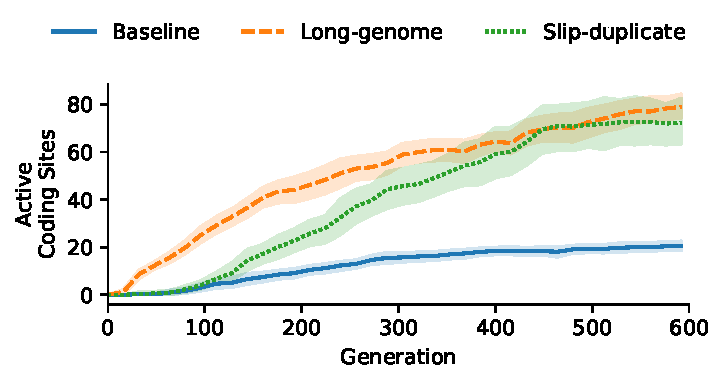
\includegraphics[width=\linewidth]{binder/binder/teeplots/hue=treatment+post=plt-xlim-0-600+viz=lineplot+x=generation-born+y=num-coding-sites+ext=.pdf}
    \caption{\footnotesize number coding sites (critical for tasks)}
    \label{fig:num-coding-sites:coding}
    \end{subfigure}

    \begin{subfigure}{\linewidth}
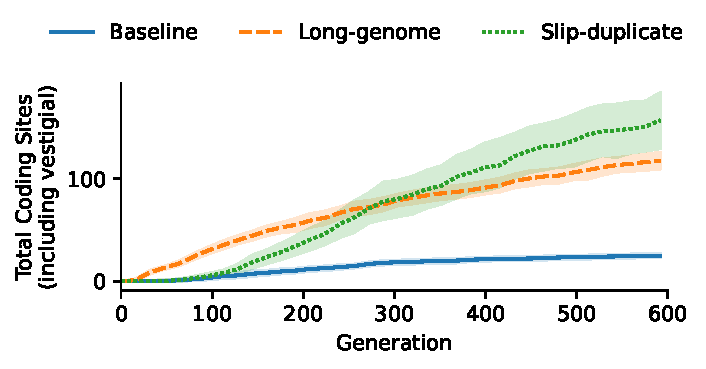
\includegraphics[width=\linewidth,]{binder/binder/teeplots/hue=treatment+post=plt-xlim-0-600+viz=lineplot+x=generation-born+y=num-coded-sites+ext=.pdf}
    \caption{\footnotesize number of sites that currently or have coded for a task}
    \label{fig:num-coding-sites:coded}
    \end{subfigure}
    \caption{
        \textbf{Growth trajectories of brittleness and coding site counts over evolutionary time.}
        \footnotesize
        Error bands give 95\% CI, bootstrapped over 30 replicates per treatment.
    }
    \label{fig:num-coding-sites}
\end{figure}



In a final set of analyses, we broadened our scope to assess consequences of gene duplication with respect to whole-genome architecture.
In particular, genome robustness, which we defined in terms of sensitivity of fitness to mutation \citep{lenski1999genome}.
We quantified robustness by measuring the number of ``critical'' genome sites, where a single-site knockout underrated replicator viability or one or more adaptive phenotypic traits (i.e., Logic-9 tasks).
\footnote{%
Although sufficiently representative for our purposes, limitations exist in detecting Avida genome functionality through single-site knockouts; such an approach can underestimate aspects of genome sequence complexity involving small effects or redundancy \citep{lenski1999genome,moreno2024cryptic}.
}

One conventional perspective on gene duplication is \textit{vis-a-vis} neutral dynamics, wherein copied genetic material reduces brittleness by introducing redundancy \citep{wagner1996genetic}.
To assess the relevance of this model within our study system, we performed slip-duplicate mutational assays to quantify the baseline effect of slip insertion mutations on robustness, in the absence of selection.

We applied our assay to final-dominant genome lineages evolved with slip duplication.
For this purpose, we generated one slip duplication per genome, and filtered away those that affected self-replication viability or altered the Logic-9 phenotype.
We then measured change in critical site counts between corresponding wildtype and mutated variants.

Fitness-neutral slip insertions did indeed tend to reduce the number of genome sites detectable as a single point of failure for performed tasks.
% https://github.com/chaynes2019/AvidaGeneDupe/blob/9fee1f13a8d31f25d1dd799c6a26f9b7fa617738/binder/indel-effect-nulldist.ipynb
On average, we found that neutral slip insertions decreased coding site count by 6.8 sites (bootstrapped 95\% CI 6.4 to 7.3).
This effect was strongest in genomes with high complexity; for instance, neutral insertion mutations decrease coding site count by 9.2 and 8.3 sites on average in genomes that encode 4- and 5-component complexity tasks, respectively (bootstrapped 95\% CIs 8.5 to 9.9 and 7.2 to 9.3).
Supplementary Figure \ref{fig:nulldist} presents these results.

% https://github.com/chaynes2019/AvidaGeneDupe/blob/binder/binder/gain-mechanism.ipynb
To assess evolutionary consequences of redundancies introduced by slip-duplication, we next pivoted to assess coding site accumulation within genomes over the course of evolution.
Counter to naive expectation, we found that the slip duplication treatment accrued fitness-critical sites at a generation-on-generation rate comparable to the long-genome baseline treatment (Figure \ref{fig:num-coding-sites:coding}; Mann-Whittney test, $U=361$, $p=0.19$; second-phase experiments).
Despite this similarity, however, when measurements were taken inclusive of vestigial coding sites (those which had \textit{previously} been fitness-critical earlier within a lineage), we found a significantly increased coding site count associated with the slip-duplicate treatment (Mann-Whittney test, $U=630$, $p<0.01$; second-phase experiments).
Figure \ref{fig:num-coding-sites:coded} compares vestigial-inclusive coding site counts trajectories along final-dominant lineages.
It therefore appears that slip duplication processes within our study system act to increase the net supply of coding material in the genome available to neutral processes, but do not suppress accumulation of genome brittleness.

% One possible explanation is that selective pressures are driving the two treatments to reach a similar number of critical sites, but slip duplication can duplicate and copy genome content in a manner that increases the copy count of previously coding sites relative to the number of critical sites.
